% flashcards-title: Marked centimeter scale
% flashcards-desc: A high-contrast scale runs from zero to five centimeters. Each centimeter is divided into ten equal minor intervals, with a distinct half-centimeter mark.
\documentclass[border=5mm]{standalone}
\def\pgfsysdriver{pgfsys-dvisvgm.def}
\usepackage{tikz}
\usetikzlibrary{arrows.meta,calc,patterns.meta,positioning}
\renewcommand{\familydefault}{\sfdefault}

\definecolor{fcInk}{HTML}{1C1C1E}
\definecolor{fcMuted}{HTML}{68686D}
\definecolor{fcGuide}{HTML}{C9C9CE}
\definecolor{fcGold}{HTML}{D7A313}
\definecolor{fcGoldSoft}{HTML}{F8E8AE}

\tikzset{
  fc canvas/.style={fill=white, rounded corners=2.5mm},
  fc vector/.style={
    draw=fcGold,
    line width=1.35mm,
    line cap=round,
    -{Stealth[length=4.1mm,width=3.25mm]}
  },
  fc vector secondary/.style={
    draw=fcInk,
    line width=1.15mm,
    line cap=round,
    dash pattern=on 4.1mm off 2.6mm,
    -{Stealth[length=3.9mm,width=3.1mm]}
  },
  fc resultant/.style={
    draw=fcMuted,
    line width=1.55mm,
    line cap=round,
    -{Stealth[length=4.6mm,width=3.6mm]}
  },
  fc axis/.style={
    draw=fcInk,
    line width=.72mm,
    -{Stealth[length=3.1mm,width=2.5mm]}
  },
  fc guide/.style={
    draw=fcMuted,
    line width=.55mm,
    dash pattern=on 2.3mm off 1.8mm
  },
  fc construction/.style={draw=fcGuide, line width=.32mm},
  fc endpoint/.style={circle, fill=fcInk, inner sep=1.45mm},
  fc label/.style={font=\bfseries\large, text=fcInk},
  fc small label/.style={font=\small, text=fcMuted},
  fc caption/.style={font=\bfseries\small, text=fcMuted}
}

\begin{document}
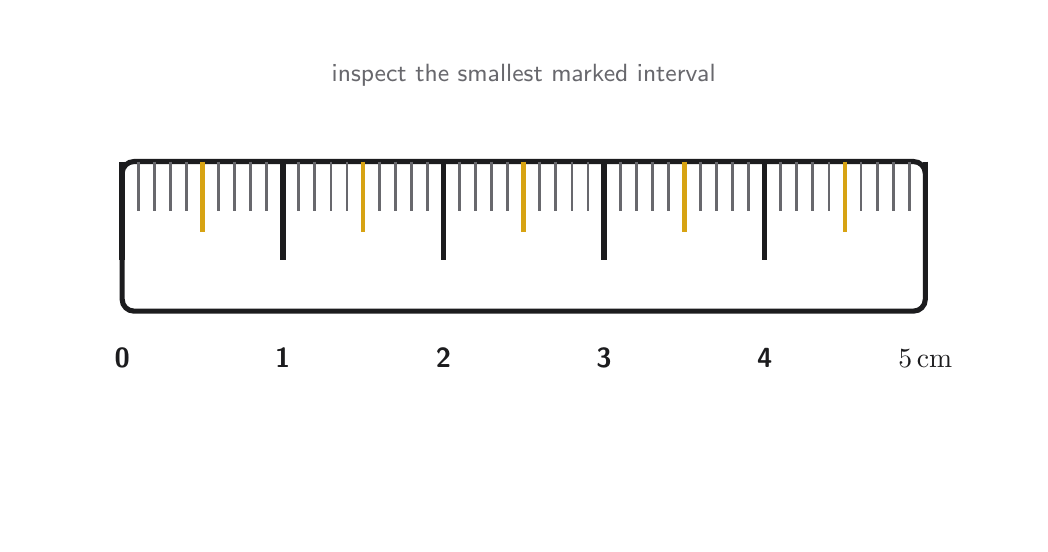
\begin{tikzpicture}[x=1cm,y=1cm]
  \path[fc canvas] (-.45,-.45) rectangle (12.15,5.85);
  \node[fc small label] at (5.85,5.25) {inspect the smallest marked interval};

  \path[draw=fcInk, fill=white, line width=.65mm, rounded corners=1.5mm]
    (.75,2.25) rectangle (10.95,4.15);
  \foreach \i in {0,...,50} {
    \pgfmathsetmacro{\x}{.75 + .204*\i}
    \pgfmathtruncatemacro{\major}{mod(\i,10)}
    \pgfmathtruncatemacro{\half}{mod(\i,5)}
    \ifnum\major=0
      \draw[draw=fcInk, line width=.7mm] (\x,4.15) -- (\x,2.9);
    \else
      \ifnum\half=0
        \draw[draw=fcGold, line width=.58mm] (\x,4.15) -- (\x,3.25);
      \else
        \draw[draw=fcMuted, line width=.36mm] (\x,4.15) -- (\x,3.52);
      \fi
    \fi
  }
  \foreach \i in {0,...,5} {
    \pgfmathsetmacro{\x}{.75 + 2.04*\i}
    \node[font=\bfseries\normalsize, text=fcInk] at (\x,1.65)
      {\ifnum\i=5 $5\,\mathrm{cm}$\else\i\fi};
  }
\end{tikzpicture}
\end{document}
